\chapter{Estimating DSGE models - basics} \label{ch:estbase}

As in the chapter \ref{ch:solbase}, this chapter is structured around an example. The goal of this chapter is to lead you through the basic functionality in Dynare to estimate models using Bayesian techniques, so that by the end of the chapter you should have the capacity to estimate a model of your own. This chapter is therefore very practically-oriented and abstracts from the underlying computations that Dynare undertakes to estimate a model; that subject is instead covered in some depth in Chapter \ref{ch:estadv} on advanced topics. \\

\section{Introducing the example} \label{sec:modsetup}
The example that we will follow in some details in this chapter is drawn from \citet{Schorfheide2000}. This first section introduces the model, its basic intuitions and equations. We will then see in subsequent sections how to estimate it using Dynare. Note that the original paper by Schorfheide mainly focusses on estimation methodologies, difficulties and solutions, with a special interest in model comparison, while the mathematics and economic intuitions of the model it evaluates are drawn from, and left to, \citet{CogleyNason1994}. If anything is left unanswered or vague in the description below, you may also want to refer to \citet{CogleyNason1994}.\\

In essence, the model studied by \citet{Schorfheide2000} is one of cash in advance (CIA). The goal of the paper is to estimate the model using Bayesian techniques, while observing only output and inflation. In the model, there are several markets and actors to keep track of. So to clarify things, figure \ref{fig:schorfmod} sketches the main dynamics of the model. As we go through the set-up of the model, you may find it helpful to refer back to the figure. 
\begin{figure} \label{fig:schorfmod}
\begin{center} 
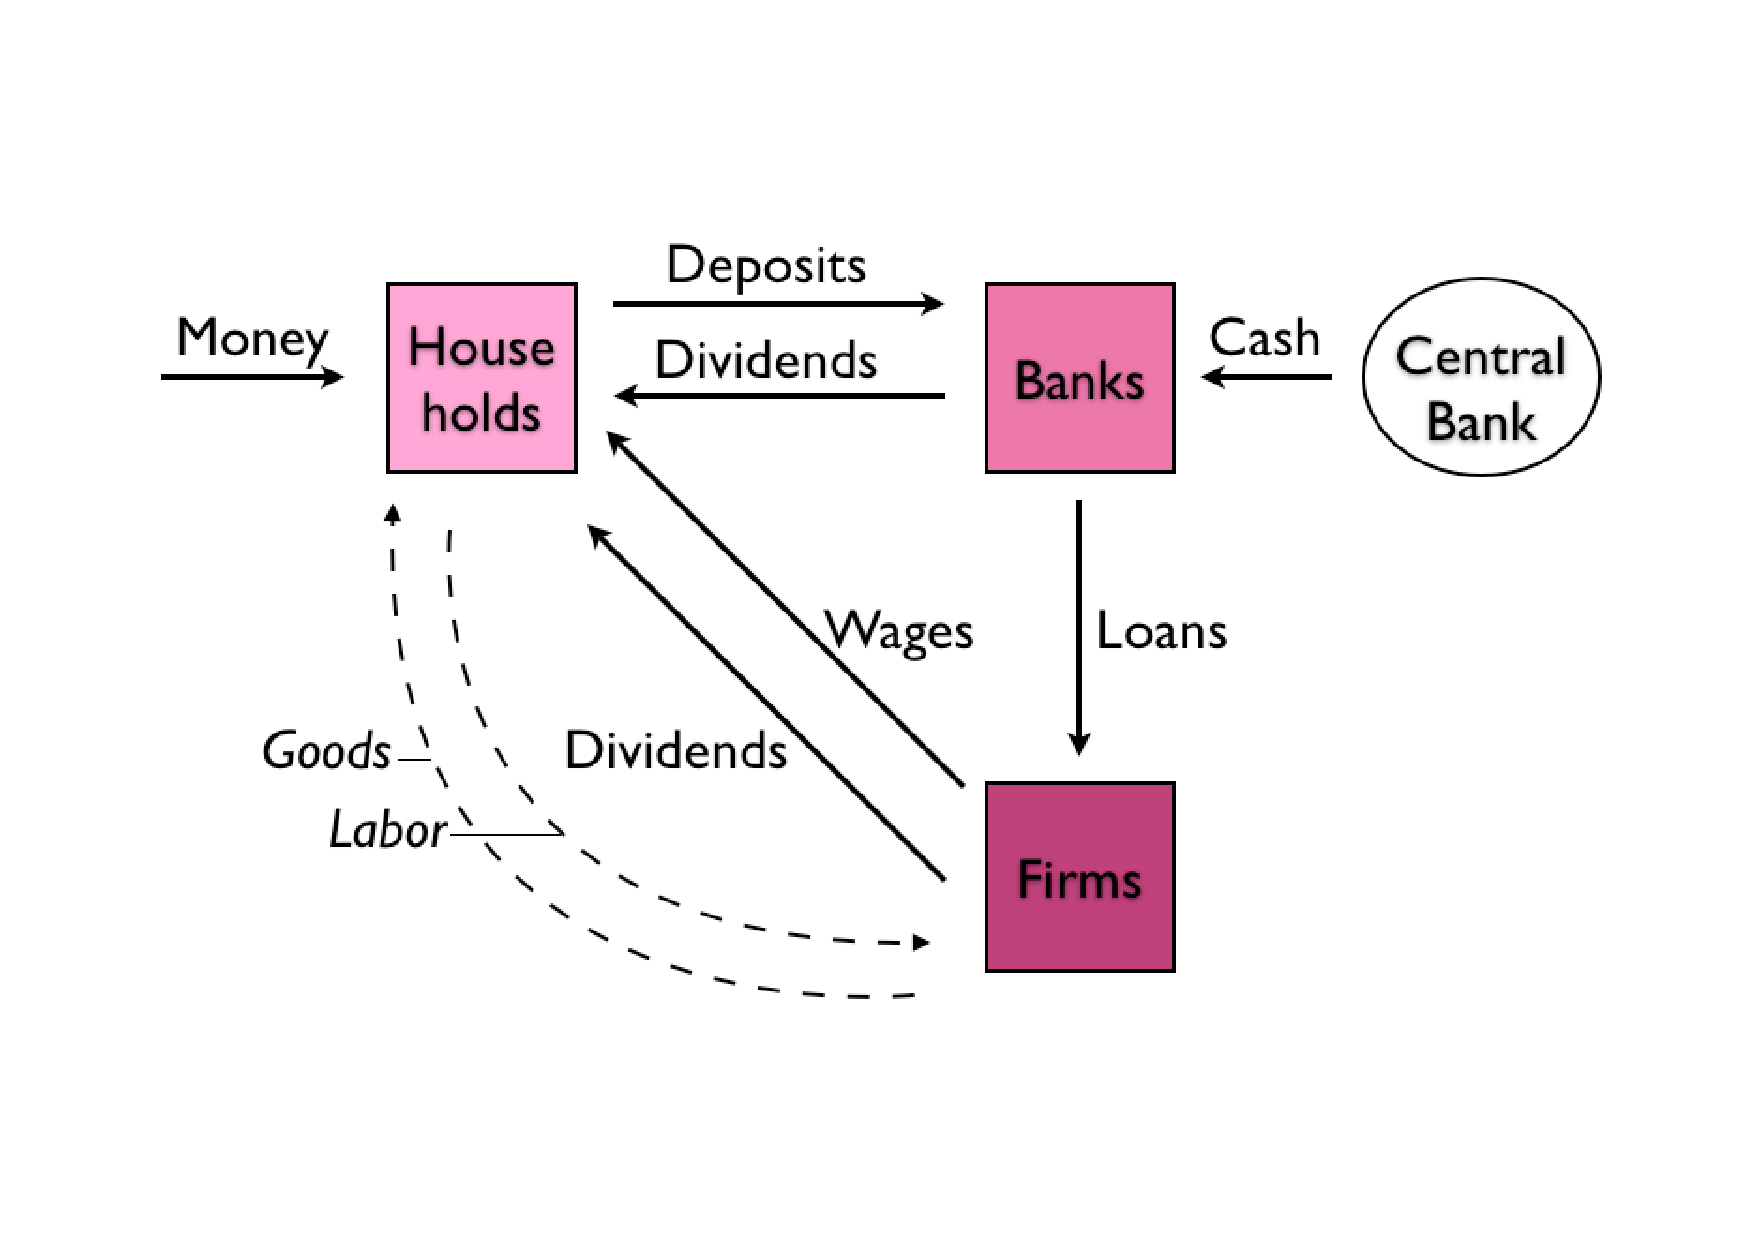
\includegraphics[width=1.0\textwidth]{P_SchorfMod} 
\end{center} 
\caption[CIA model illustration]{Continuous lines show the circulation of nominal funds, while dashed lines show the flow of real variables.} 
\end{figure}\\

The economy is made up of three central agents and one secondary agent: households, firms and banks (representing the financial sector), and a monetary authority which plays a minor role. Households maximize their utility function which depends on consumption, $C_t$, and hours worked, $H_t$, while deciding how much money to hold next period in cash, $M_{t+1}$ and how much to deposit at the bank, $D_t$, in order to earn $R_{H,t}-1$ interest. Households therefore solve the problem
\begin{eqnarray*}
\substack{\max \\ \{C_t,H_t,M_{t+1},D_t\}} & \mathbb{E}_0 \left[ \sum_{t=0}^\infty \beta^t \left[ (1-\phi) \ln C_t + \phi \ln (1-H_t) \right] \right] \\
\textrm{s.t.} & P_t C_t \leq M_t - D_t + W_t H_t \\
& 0 \leq D_t \\
& M_{t+1} = (M_t - D_t + W_tH_t - P_tC_t) + R_{H,t}D_t + F_t + B_t
\end{eqnarray*}
where the second equation spells out the cash in advance constraint including wage revenues, the third the inability to borrow from the bank and the fourth the intertemporal budget constraint emphasizing that households accumulate the money that remains after bank deposits and purchases on goods are deducted from total inflows made up of the money they receive from last period's cash balances, wages, interests, as well as dividends from firms, $F_t$ and from banks, $B_t$ which in both cases are made up of net cash inflows defined below. \\

Banks, on their end, receive cash deposits from households and a cash injection, $X_t$ from the central bank (which equals the net change in nominal money balances, $M_{t+1}-M_t$). It uses these funds to disburse loans to firms, $L_t$, on which they make a net return of $R_{F,t}-1$. Of course, banks are constrained in their loans by a credit market equilibrium condition $L_t \leq X_t + D_t$. Finally, bank dividends, $B_t$ are simply equal to $D_t + R_{F,t}L_t - R_{H,t}D_t - L_t + X_t$. \\

Finally, firms maximize the net present value of future dividends (discounted by the marginal utility of consumption, since they are owned by households) by choosing dividends, next period's capital stock, $K_{t+1}$, labor demand, $N_t$ and loans. Its problem is summarized by
\begin{eqnarray*}
\substack{\max \\ \{F_t,K_{t+1},N_{t},L_t\}} & \mathbb{E}_0 \left[ \sum_{t=0}^\infty \beta^{t+1} \frac{F_t}{C_{t+1}P_{t+1}} \right] \\
\textrm{s.t.} & F_t \leq L_t + P_t \left[ K_t^\alpha (A_t N_t)^{1-\alpha} - K_{t+1} + (1-\delta)K_t \right] - W_tN_t-L_tR_{F,t} \\
& W_tN_t \leq L_t\\
\end{eqnarray*}
where the second equation makes use of the production function \mbox{$Y_t = K_t^\alpha (A_t N_t)^{1-\alpha}$} and the real aggregate accounting constraint (goods market equilibrium) \mbox{$C_t + I_t = Y_t$}, where $I_t=K_{t+1} - (1-\delta)K_t$, and where $\delta$ is the rate of depreciation. Note that it is the firms that engage in investment in this model, by trading off investment for dividends to consumers. The third equation simply specifies that bank loans are used to pay for wage costs. \\

To close the model, we add the usual labor and money market equilibrium equations, $H_t= N_t$ and $P_tC_t=M_t + X_t$, as well as the condition that $R_{H,t}=R_{F,t}$ due to the equal risk profiles of the loans.\\

More importantly, we add the stochastic elements to the model. The model allows for two sources of perturbations, one real affecting technology and one nominal affecting the money stock. These important equations are
\[
\ln A_t = \gamma + \ln A_{t-1} + \epsilon_{A,t}, \qquad \epsilon_{A,t} \thicksim N(0,\sigma_A^2)
\]
and

\[
\ln m_t = (1-\rho)\ln m^* + \rho \ln m_{t-1} + \epsilon_{M,t}, \qquad \epsilon_{M,t} \thicksim N(0,\sigma_M^2)
\]
where $m_t \equiv M_{T+1}/M_t$ is the growth rate of the money stock.\\

The first equation is therefore a unit root with drift in the log of technology, and the second an autoregressive stationary process in the growth rate of money, but an AR(2) in the level of money which has a unit root in the log of the level of money. (You can convince yourself of this by writing the AR(2) process in state space form and realizing that the system has an eigenvalue of one. Alternatively, one is a root of the second order autoregressive lag polynomial. As usual, if the logs of a variable are specified to follow a unit root process, the rate of growth of the series is a stationary stochastic process; see \citet{Hamilton1994}, chapter 15, for details.)\\

When the above functions are maximized, we obtain the following set of first order and equilibrium conditions. We will not dwell on the derivations here, to save space, but encourage you to browse \citet{CogleyNason1994} for additional details. We nonetheless give a brief intuitive explanation of each equation. The system comes down to
\begin{eqnarray*}
\mathbb{E}_{t}\bigg\{-\widehat{P}_{t}/\left[ \widehat{C}_{t+1}\widehat{P}_{t+1}m_{t}%
\right]\bigg\}&=&\beta e^{-\alpha (\gamma +\varepsilon_{t+1})}P_{t+1}\Big[\alpha\widehat{K}_{t}^{\alpha -1}N_{t+1}^{1-\alpha }+
(1-\delta )\Big]\\
&&/\left[ 
\widehat{c}_{t+2}\widehat{P}_{t+2}m_{t+1}\right] \bigg\}\\
\widehat{W}_{t}&=&\widehat{L}_{t}/N_{t}\\
\frac{\phi }{1-\phi }\left[ \widehat{C}_{t}\widehat{P}_{t}/\left(
1-N_{t}\right) \right]&=&\widehat{L}_{t}/N_{t}\\
R_{t}&=&(1-\alpha )\widehat{P}_{t}e^{-\alpha (\gamma +\varepsilon_{t+1})}\widehat{K}_{t-1}^{\alpha}N_{t}^{-\alpha }/\widehat{W}_{t}\\
\left[ \widehat{C}_{t}\widehat{P}_{t}\right] ^{-1}&=&\beta \left[ \left(
1-\alpha \right) \widehat{P}_{t}e^{-\alpha (\gamma +\varepsilon_{t+1})}\widehat{K}_{t-1}^{\alpha}N_{t}^{1-\alpha }
\right]\\
&& \times  \mathbb{E}_{t}\left[\widehat{L}_{t}m_{t}\widehat{C}_{t+1}\widehat{P}_{t+1}\right] ^{-1}\\
\widehat{C}_t+\widehat{K}_t &=& e^{-\alpha(\gamma+\varepsilon_t)}\widehat{K}_{t-1}^\alpha N^{1-\alpha}+(1-\delta)e^{-(\gamma+\varepsilon_t)}\widehat{K}_{t-1}\\
\widehat{P}_t\widehat{C} &=& m_t\\
m_t-1+\widehat{D}_t &=& \widehat{L}_t\\
\widehat{Y}_t &=& \widehat{K}_{t-1}^\alpha N^{1-alp}e^{-\alpha (\gamma+\varepsilon_t)}\\
\ln(m_t) &=& (1-\rho)\ln(m^\star) + \rho\ln(m_{t-1})+\eta_t\\
\frac{A_t}{A_{t-1}}  \equiv  dA_t & = & \exp( \gamma + \epsilon_{A,t})\\
Y_t/Y_{t-1} &=& e^{\gamma+\varepsilon_t}\widehat{Y}_t/\widehat{Y}_{t-1}\\
P_t/P_{t-1} &=& (\widehat{P}_t/\widehat{P}_{t-1})(m_{t-1}/e^{\gamma+\varepsilon_t})
\end{eqnarray*}
where, importantly, hats over variables no longer mean deviations from steady state, but instead represent variables that have been made stationary. We come back to this important topic in details in section \ref{sec:decmod} below on declaring the model in Dynare. For now, we pause a moment to give some intuition for the above equations. In order, these equations correspond to:
\begin{enumerate}
\item The Euler equation in the goods market, representing the tradeoff to the economy of moving consumption goods across time.
\item The firms' borrowing constraint, also affecting labor demand, as firms use borrowed funds to pay for labor input.
\item The intertemporal labor market optimality condition, linking labor supply, labor demand, and the marginal rate of substitution between consumption and leisure. 
\item The equilibrium interest rate in which the marginal revenue product of labor equals the cost of borrowing to pay for that additional unit of labor.
\item The Euler equation in the credit market, which ensures that giving up one unit of consumption today for additional savings equals the net present value of future consumption.
\item The aggregate resource constraint.
\item The money market equilibrium condition equating nominal consumption demand to money demand to money supply to current nominal balances plus money injection. 
\item The credit market equilibrium condition.
\item The production function.
\item The stochastic process for money growth.
\item The stochastic process for technology.
\item The relationship between observable variables and stationary variables; more details on these last two equations appear in the following section. 
\end{enumerate}

\section{Declaring variables}
To input the above model into Dynare for estimation purposes, we must first declare the mode's variables. This is done exactly as described in chapter \ref{ch:solbase} on solving DSGE models. We thus begin the .mod file with:\\
\\
\texttt{var m P c e W R k d n l gy\_obs gp\_obs Y\_obs P\_obs y dA; \\
varexo e\_a e\_m;}\\
\\
where the choice of upper and lower case letters is not significant, the first set of endogenous variables, up to $l$, are as specified in the model setup above, and where the last five variables are defined and explained in more details in the section below on declaring the model in Dynare. The exogenous variables are as expected and concern the shocks to the evolution of technology and  money balances. \\

\section{Declaring the model: from theory to Dynare} \label{sec:decmod}

The problem that must first be addressed is the non-stationarity of the variables originating from the stochastic trends in technology and money growth. In order to linearize and solve the DSGE model - a necessary first step before estimating it - we must have a steady state. Thus, we must write the model using stationary variables. Our task will then be to link these stationary variables to the data which, according to the basic (non-stationary) model, is non-stationary. Of course, we have the option to stationarize the data by looking at growth rates instead of levels, but can also work with non-stationary data in levels. The latter complicates things somewhat, but illustrates several features of Dynare worth highlighting; we therefore elect this path in our example below. But again, independently of the data, the model we input into Dynare must contain stationary variables, except for the observable variables. \\

Let us then first focus on this problem of non-stationarity. It is possible to show, by solving the above model, that it does not have a steady state. Instead, when shocks are null, real variables growth with $A_t$ (except for labor, $N_t$, which is stationary as there is no population growth), nominal variables grow with $M_t$ and prices with $M_t/A_t$. Stochastic detrending therefore involves the following operations (where hats over variables represent stationary variables). For real variables, $\hat q_t=q_t/A_t$, where $q_t = [y_t, c_t, i_t, k_{t+1} ]$. For nominal variables, $\hat{Q}_t = Q_t/M_t$, where $Q_t = [ d_t, l_t, W_t ]$. And for prices, $\hat P_t = P_t \cdot A_t / M_t$. \\

Let's illustrate this transformation on output, and leave the transformations of the remaining equations as an exercise (\citet{CogleyNason1994} includes more details on the transformations of each equation). We stationarize output by dividing its real variables (except for labor) by $A_t$. We define $\widehat{Y}_t$ to equal $Y_t / A_t$ and $\widehat{K}_t$ as $K_t / A_t$. \textsf{\textbf{TIP!}} Note, though, that in Dynare, the stock variables adopt the time subscript of the period in which they are decided (for more details, see section \ref{sec:modspe} in chapter \ref{ch:solbase}). Thus, in the output equation, we should actually work with $\widehat{K}_{t-1}=K_{t-1} / A_{t-1}$. The resulting equation made up of stationary variables is
\begin{eqnarray*}
\frac{Y_t}{A_t} & = & \left( \frac{K_{t-1}}{A_{t-1}} \right)^\alpha A_t^{1-\alpha} N_t^{1-\alpha} A_t^{-1} A_{t-1}^\alpha \\
\widehat{Y}_t & = & \widehat{K}_{t-1}^\alpha N_t^{1-\alpha} \left( \frac{A_t}{A_{t-1}} \right)^{-\alpha} \\
& = & \widehat{K}_{t-1}^\alpha N_t^{1-\alpha} \exp(-\alpha (\gamma + \epsilon_{A,t}))
\end{eqnarray*}
where we go from the second to the third line by taking the exponential of both sides of the equation of motion of technology.\\

The above is the equation we retain for the .mod file of Dynare into which we type:\\
\\
\texttt{y=k(-1)$\hat{}$alp*n$\hat{}$(1-alp)*exp(-alp*(gam+e\_a))}\\
\\

The other equations are entered into the .mod file after transforming them in exactly the same way as the one above. But before presenting all final equations, let's consider two additional transformations. First, since we often deal with the growth rate of technology, we specify the equation of motion of technology as\\
\\
\texttt{dA = exp(gam+e\_a)}\\
\\
by simply taking the exponential of both sides of the stochastic process of technology defined in the model setup above. \\

And finally, we must make a decision as to what we do with our non-stationary observations. We could simply stationarize them by looking at the rates of growth (which we know are constant). In the case of output, the observable variable would become $Y_t /Y_{t-1}$. We would then have to relate this to our stationary variables by using the definition that $\widehat{Y}_t \equiv Y_t/ A_t$:\\
\\
\texttt{gy\_obs = dA*y/y(-1);}\\
\\

But, as we suggested earlier, since we want to work with the non-stationary series directly, we separate out $Y_t$ and $Y_{t-1}$ in the above, and making use of the identity $Y_t/Y_{t-1}=(\widehat{Y}_t/\widehat{Y}_{t-1})\cdot \exp (\gamma + \epsilon_{A,t})$, we add to the .mod file\\
\\
\texttt{Y\_obs/Y\_obs(-1) = gy\_obs}\\
\\
We of course do the same for prices, our other observable variable, except that prices grow with $M_t/A_t$ as noted earlier. The details of the correct transformations for prices are left as an exercise.\\

The resulting model block of the .mod file is therefore:\\
\\
\texttt{model;\\
dA = exp(gam+e\_a);\\
log(m) = (1-rho)*log(mst) + rho*log(m(-1))+e\_m;\\
-P/(c(+1)*P(+1)*m)+bet*P(+1)*(alp*exp(-alp*(gam+log(e(+1))))*k$\hat{}$(alp-1)\\
*n(+1)$\hat{}$(1-alp)+(1-del)*exp(-(gam+log(e(+1)))))/(c(+2)*P(+2)*m(+1))=0;\\
W = l/n;\\
-(psi/(1-psi))*(c*P/(1-n))+l/n = 0;\\
R = P*(1-alp)*exp(-alp*(gam+e\_a))*k(-1)$\hat{}$alp*n$\hat{}$(-alp)/W;\\
1/(c*P)-bet*P*(1-alp)*exp(-alp*(gam+e\_a))*k(-1)$\hat{}$alp*n$\hat{}$(1-alp)/(m*l*c(+1)*P(+1)) = 0;\\
c+k = exp(-alp*(gam+e\_a))*k(-1)$\hat{}$alp*n$\hat{}$(1-alp)+(1-del)*exp(-(gam+e\_a))*k(-1);\\
P*c = m;\\
m-1+d = l;\\
e = exp(e\_a);\\
y = k(-1)$\hat{}$alp*n$\hat{}$(1-alp)*exp(-alp*(gam+e\_a));\\
gy\_obs = dA*y/y(-1);\\
gp\_obs = (p/p(-1))*m(-1)/dA;\\
Y\_obs/Y\_obs(-1) = gy\_obs;\\
P\_obs/P\_obs(-1) = gp\_obs;\\
end;}\\
\\
where, of course, the input conventions, such as ending lines with semicolons and indicating the timing of variables in parentheses, are the same as those listed in chapter \ref{ch:solbase}. \\

\section{Specifying variable characteristics}
A natural extension of our discussion above is to declare, in Dynare, which variables are observable and which are non-stationary. We begin with the first and declare, in our .mod file\\
\\
\texttt{varobs P\_obs Y\_obs;}\\
\\
to specify that our observable variables are indeed P\_obs and Y\_obs as noted in the section above. \textsf{\textbf{TIP!}} Note that the number of unobserved variables (number of \texttt{var} minus number of \texttt{varobs}) must be smaller or equal to the number of shocks such that the model be estimated. If this is not the case, you should add measurement shocks to your model where you deem most appropriate. \\

Secondly, we also recall that we decided to work with the levels of these variables, which are not stationary. In fact, both exhibit stochastic trends. This can be seen explicitly by taking the difference of logs of output and prices to compute growth rates. In the case of output, we make use of the fact that $Y_t=\widehat Y_t \cdot A_t$. Taking logs of both sides and subtracting the same equation scrolled back one period, we find:
\[
\Delta \ln Y_t = \Delta \ln \widehat Y_t + \gamma + \epsilon_{A,t}
\]
emphasizing clearly the drift term $\gamma$, whereas we know $\Delta \ln \widehat Y_t$ is stationary in steady state. \\

In the case of prices, we apply the same manipulations to show that:
\[
\Delta \ln P_t = \Delta \ln \widehat P_t + \ln m_{t-1} - \gamma - \epsilon_{A,t}
\]
again, highlighting the trend terms clearly. \\

In Dynare, these trends must be declared up front. We therefore write\\
\\
\texttt{observation\_trends;\\
P\_obs (log(exp(gam)/mst));\\
Y\_obs (gam);\\
end;}\\
(** not sure I get the trend declaration for prices... how does it match the growth rate computed above? mst is simply the steady state growth of m?). In general, the command \texttt{observation\_trends} specifies linear trends as a function of model parameters for the observed variables in the model.\\

And finally, since P\_obs and Y\_obs inherit the unit root characteristics of their driving variables, technology and money, we must tell Dynare to use a diffuse prior (infinite variance) for their initialization in the Kalman filter. Note that for stationary variables, the unconditional covariance matrix of these variables is used for initialization. The algorithm to compute a true diffuse prior is taken from \citet{DurbinKoopman2001}. To give these instructions to Dynare, we write in the .mod\\
\\
\texttt{options\_.unit\_root\_vars = \{'P\_obs'; 'Y\_obs' \};}\\
\\
(** is this only if we have a true unit root, or also if we have non-stationarity coming from a deterministic trend, for instance?)\\

\section{Specifying the steady state}
Before Dynare estimates a model, it first linearizes it around a steady state. Thus, a steady state must exist for the model and although Dynare can calculate it, we must give it a hand by declaring approximate values for the steady states. This is just as explained in details and according to the same syntax explained in chapter \ref{ch:solbase}, with the convenient options to use the commands \texttt{steady} and \texttt{check}. The only difference with regards to model estimation is the non-stationary nature of our observable variables. In this case, the declaration of the steady state must be slightly amended in Dynare. (** fill in with the new functionality from Dynare version 4, currently the answer is to write a separate Matlab file which solves the steady state for the stationary variables and returns dummies for the non stationary variables). 

\section{Declaring priors}
Priors play an important role in Bayesian estimation and consequently deserve a central role in the specification of the .mod file. Priors, in Bayesian estimation, are declared as a distribution. The general syntax to introduce priors in Dynare is the following:\\
\\
\texttt{estimated\_params;\\
PARAMETER NAME, PRIOR\_SHAPE, PRIOR\_MEAN, PRIOR\_STANDARD\_ERROR [, PRIOR 3$^{\textrm{rd}}$ PARAMETER] [,PRIOR 4$^{\textrm{th}}$ PARAMETER] ; \\
end; }\\
\\
where the following table defines each term more clearly\\
\\
    \begin{tabular}{llc}
    \textbf{\underline{PRIOR\_SHAPE}} & \textbf{\underline{Corresponding distribution}} & \textbf{\underline{Range}} \\
      NORMAL\_PDF & $N(\mu,\sigma)$ & $\mathbb{R}$\\
      GAMMA\_PDF &  $G_2(\mu,\sigma,p_3)$ & $[p_3,+\infty)$\\
        BETA\_PDF & $B(\mu,\sigma,p_3,p_4)$ & $[p_3,p_4]$\\
        INV\_GAMMA\_PDF & $IG_1(\mu,\sigma)$ & $\mathbb R^+$\\
UNIFORM\_PDF& $U(p_3,p_4)$ &  $[p_3,p_4]$
    \end{tabular}\\
    \\
    \\
    where $\mu$ is the \texttt{PRIOR\_MEAN}, $\sigma$ is the \texttt{PRIOR\_STANDARD\_ERROR}, $p_3$ is the \texttt{PRIOR 3$^{\textrm{rd}}$ PARAMETER} (whose default is 0) and $p_4$ is the \texttt{PRIOR 4$^{\textrm{th}}$ PARAMETER} (whose default is 1). \\
    
For a more complete review of all possible options for declaring priors, as well as the syntax to declare priors for maximum likelihood estimation (not Bayesian), see the Reference Manual (** add link). Note also that if some parameters in a model are calibrated and are not to be estimated, you should declare them as such, by using the \texttt{parameters} command and its related syntax, as explained in chapter \ref{ch:solbase}. \\
    
\textsf{\textbf{TIP!}} It may at times be desirable to estimate a transformation of a parameter appearing in the model, rather than the parameter itself. In such a case, it is possible to declare the parameter to be estimated in the parameters statement and to define the transformation at the top of the model section, as a Matlab expression, by adding a pound sign (\#) at the beginning of the corresponding line. For example:\\
\\
\texttt{model;\\
      \# sig = 1/bet;\\
      c = sig*c(+1)*mpk;\\
      end;\\
\\
      estimated\_params;\\
      bet,normal\_pdf,1,0.05;\\
      end;}\\

\textsf{\textbf{TIP!}} Finally, another useful command to use is the \texttt{estimated\_params\_init} command which declares numerical initial values for the optimizer when these one are different from the prior mean. This is especially useful when redoing an estimation - if the optimizer got stuck the first time around, or if the number of Metropolis-Hastings draws was insufficient - and wanting to enter the posterior mode as initial values for the parameters instead of a prior. The Reference Manual (** add link) gives more details as to the exact syntax of this command.\\

Coming back to our example and having learned how to enter priors, we expand our .mod file with the following information: \\
\\
\texttt{estimated\_params;\\
alp, beta\_pdf, 0.356, 0.02; \\ 
bet, beta\_pdf, 0.993, 0.002; \\
gam, normal\_pdf, 0.0085, 0.003; \\
mst, normal\_pdf, 1.0002, 0.007; \\
rho, beta\_pdf, 0.129, 0.223;\\
psi, beta\_pdf, 0.65, 0.05;\\
del, beta\_pdf, 0.01, 0.005;\\
stderr e\_a, inv\_gamma\_pdf, 0.035449, inf;\\
stderr e\_m, inv\_gamma\_pdf, 0.008862, inf;\\
end;}\\
\\
(** do you still need to declare all parameters using the ``parameter'' command at the top of the .mod file?)\\

\section{Initiating the estimation} \label{sec:estimate}
To ask Dynare to estimate a model, all that is necessary is to add the command \texttt{estimation} at the end of the .mod file. Easy enough. But the real complexity comes from the options available for the command (to be entered in parentheses and sequentially, separated by commas, after the command \texttt{estimation}). Below, we list the most common and useful options, and encourage you to view the Reference Manual (** add link) for a complete list. \\
\begin{enumerate}
\item datafile = FILENAME: the datafile (a .m file, a .mat file, or an .xls file). Note that observations do not need to show up in any order, but vectors of observations need to be named with the same names as those in \texttt{var\_obs}. In Excel files, for instance, observations could be ordered in columns, and variable names would show up in the first cell of each column.
\item nobs = INTEGER: the number of observations to be used (default: all observations in the file) 
\item first\_obs = INTEGER: the number of the first observation to be used (default = 1). This is useful when running loops, or instance, to divide the observations into sub-periods. 
\item prefilter = 1: the estimation procedure demeans the data (default=0, no prefiltering). This is useful if model variables are in deviations from steady state, for instance, and therefore have zero mean. Demeaning the observations would also impose a zero mean on the observed variables.  
\item nograph: no graphs should be plotted.
\item lik\_init: INTEGER: type of initialization of Kalman filter. 
\subitem 1 (default): for stationary models, the initial matrix of variance of the error of forecast is set equal to the 
unconditional variance of the state variables. 
\subitem 2: for nonstationary models: a wide prior is used with an initial matrix of variance of the error of forecast 
diagonal with 10 on the diagonal. When using \texttt{unit\_root\_vars}, the \texttt{like\_init} option as no effect. (** but if have both stationary and nonstationary variables, what option should you use?)
\item conf\_sig = \{INTEGER | DOUBLE \}: the level for the confidence intervals reported in the results (default = 0.90) 
\item mh\_replic = INTEGER: number of replication for Metropolis Hasting algorithm. For the time being, mh\_replic 
should be larger than 1200 (default = 20000) ** is this still true? 
\item mh\_nblocks = INTEGER: number of parallel chains for Metropolis Hasting algorithm (default = 2). Despite this low default value, it is advisable to work with a higher value, such as 5 or more. This improves the computation of between group variance of the parameter means, one of the key criteria to evaluate the efficiency of the Metropolis-Hastings to evaluate the posterior distribution. More details on this subject appear in Chapter \ref{ch:estadv}.  
\item mh\_drop = DOUBLE: the fraction of initially generated parameter vectors to be dropped before using posterior 
simulations (default = 0.5) ** what does initially generated mean?
\item mh\_jscale = DOUBLE: the scale to be used for the jumping distribution in MH algorithm. The default value is 
rarely satisfactory. This option must be tuned to obtain, ideally, an accpetation rate of 25\% in the Metropolis- Hastings algorithm (default = 0.2). The idea is not to reject or accept too often a candidate parameter; the literature has settled on a value of approximately 25\%. If the acceptance rate were too high, your Metropolis-Hastings iterations would never visit the endzones of a distribution, while if it were too low, the iterations would get stuck in a subspace of the parameter range. Note that the acceptance rate drops if you increase the scale used in the jumping distribution and vice a versa.
\item mh\_init\_scale=DOUBLE: the scale to be used for drawing the initial value of the Metropolis-Hastings chain (default=2*mh\_jscale). The idea here is to draw initial values from a stretched out distribution in order to maximize the chances of these values not being too close together, which would defeat the purpose of running several blocks of Metropolis-Hastings chains.
\item mode\_file=FILENAME: name of the file containing previous value for the mode. When computing the mode, 
Dynare stores the mode (xparam1) and the hessian (hh) in a file called MODEL NAME\_mode. This is a particularly helpful option to speed up the estimation process if you have already undertaken initial estimations and have values of the posterior mode. 
\item mode\_compute=INTEGER: specifies the optimizer for the mode computation. 
\subitem 0: the mode isn�t computed. mode\_file must be specified 
\subitem 1: uses Matlab fmincon (see the Reference Manual (** add link) to set options for this command).
\subitem 2: uses Lester Ingber�s Adaptive Simulated Annealing. 
\subitem 3: uses Matlab fminunc. 
\subitem 4 (default): uses Chris Sim�s csminwel. 
\item mode\_check: when mode\_check is set, Dynare plots the posterior density for values around the computed mode 
for each estimated parameter in turn. This is helpful to diagnose problems with the optimizer. A clear indication of a problem would be that the mode is not at the trough of a distribution. 
\item load\_mh\_file: when load\_mh\_file is declared, Dynare adds to previous Metropolis-Hastings simulations instead 
of starting from scratch. Again, this is a useful option to speed up the process of estimation. 
\item nodiagnostic: doesn�t compute the convergence diagnostics for Metropolis-Hastings (default: diagnostics are computed and 
displayed). Actually seeing if the various blocks of Metropolis-Hastings runs converge is a powerful and useful option to build confidence in your model estimation. More details on these diagnostics are given in Chapter \ref{ch:estadv}.
\item bayesian\_irf: triggers the computation of the posterior distribution of impulse response functions (IRFs). The length of the IRFs are controlled by the irf option (** where, how?). The shocks at the origin of these IRFs are those estimated by Dynare. 
\item moments\_varendo: triggers the computation of the posterior distribution of the theoretical moments of the endogenous variables as in \texttt{stoch\_simul} (the posterior distribution of the variance decomposition is also included). 
\item filtered\_vars: triggers the computation of the posterior distribution of filtered endogenous variables and shocks. See the note below on the difference between filtered and smoothed shocks. 
\item smoother: triggers the computation of the posterior distribution of smoothed endogenous variables and shocks. Smoothed shocks are a reconstruction of the values of unobserved shocks over the sample, using all the information contained in the sample of observations. Filtered shocks, instead, are built only based on knowing past information. To calculate one period ahead prediction errors, for instance, you should use filtered, not smoothed variables.
\item forecast = INTEGER: computes the posterior distribution of a forecast on INTEGER periods after the end of the sample used in estimation. The corresponding graph includes one confidence interval describing uncertainty due to parameters and one confidence interval describing uncertainty due to parameters and future shocks. Note that Dynare cannot forecast out of the posterior mode. You need to run Metropolis-Hastings iterations before being able to run forecasts on an estimated model.
\item tex requests the printing of results and graphs in TeX tables and graphics that can be later directly included in Latex files (** any doc on this?)
\item All options available for stoch\_simul can simply be added to the above options, separated by commas. To view a list of these options, either see the Reference Manual (** add link) or section \ref{sec:compute} of Chapter \ref{ch:solbase}. (** how do you run stoch\_simul after estimation so that the shocks to be used in the simulation are those estimated and parameters are from the posterior mode?)
\end{enumerate}

\textsf{\textbf{TIP!}} Before launching estimation it is a good idea to make sure that your model is correctly declared, that a steady state exists and that it can be simulated for at least one set of parameter values. You may therefore want to create a test version of your .mod file. In this test file, you would comment out or erase the commands related to estimation, remove the non-stationary variables from your model and instead add a \texttt{shocks} block, make sure you have \texttt{steady} and \texttt{check} following the \texttt{initval} block if you do not have exact steady state values and run a simulation using \texttt{stoch\_simul} at the end of your .mod file. Details on model solution and simulation can be found in Chapter \ref{ch:solbase}. \\

Finally, coming back to our example, we would add the following commands to ask Dynare to run a basic estimation of our model:\\
\\
\texttt{estimation(datafile=fsdat,nobs=192,loglinear,mh\_replic=5000,\\
mh\_nblocks=5,mh\_drop=0.45,mh\_jscale=0.8);}\\

This ends our description of the .mod file.

\section{The complete .mod file}

We have seen each part of the .mod separately; it's now time to get a picture of what the complete file looks like. For convenience, the file also appears in the ``examples'' folder of your Dynare installation, under \texttt{fs2000l.mod}. (** rewrite and replace example file. Also, make sure the .mod below works given the slightly rearranged order of each block. Finally, change the initval block below with the appropriate commands for Dynare version 4, with respect to the non stationary variables). \\
\\
\texttt{var m P c e W R k d n l gy\_obs gp\_obs Y\_obs P\_obs y dA; \\
varexo e\_a e\_m;\\
\\
model;\\
dA = exp(gam+e\_a);\\
log(m) = (1-rho)*log(mst) + rho*log(m(-1))+e\_m;\\
-P/(c(+1)*P(+1)*m)+bet*P(+1)*(alp*exp(-alp*(gam+log(e(+1))))*k$\hat{}$(alp-1)\\
*n(+1)$\hat{}$(1-alp)+(1-del)*exp(-(gam+log(e(+1)))))/(c(+2)*P(+2)*m(+1))=0;\\
W = l/n;\\
-(psi/(1-psi))*(c*P/(1-n))+l/n = 0;\\
R = P*(1-alp)*exp(-alp*(gam+e\_a))*k(-1)$\hat{}$alp*n$\hat{}$(-alp)/W;\\
1/(c*P)-bet*P*(1-alp)*exp(-alp*(gam+e\_a))*k(-1)$\hat{}$alp*n$\hat{}$(1-alp)/(m*l*c(+1)*P(+1)) = 0;\\
c+k = exp(-alp*(gam+e\_a))*k(-1)$\hat{}$alp*n$\hat{}$(1-alp)+(1-del)*exp(-(gam+e\_a))*k(-1);\\
P*c = m;\\
m-1+d = l;\\
e = exp(e\_a);\\
y = k(-1)$\hat{}$alp*n$\hat{}$(1-alp)*exp(-alp*(gam+e\_a));\\
gy\_obs = dA*y/y(-1);\\
gp\_obs = (p/p(-1))*m(-1)/dA;\\
Y\_obs/Y\_obs(-1) = gy\_obs;\\
P\_obs/P\_obs(-1) = gp\_obs;\\
end;\\
\\
varobs P\_obs Y\_obs;\\
\\
observation\_trends;\\
P\_obs (log(exp(gam)/mst));\\
Y\_obs (gam);\\
end;\\
\\
options\_unit\_root\_vars = \{'P\_obs'; 'Y\_obs' \};\\
\\
initval;\\
k = 6;\\
m = mst;\\
P = 2.25;\\
c = 0.45;\\
e = 1;\\
W = 4;\\
R = 1.02;\\
d = 0.85;\\
n = 0.19;\\
l = 0.86;\\
y = 0.6;\\
gy\_obs = exp(gam);\\
gp\_obs = exp(-gam); \\
dA = exp(gam);\\
end;\\
\\
steady;\\
\\
check;\\
\\
estimated\_params;\\
alp, beta\_pdf, 0.356, 0.02; \\ 
bet, beta\_pdf, 0.993, 0.002; \\
gam, normal\_pdf, 0.0085, 0.003; \\
mst, normal\_pdf, 1.0002, 0.007; \\
rho, beta\_pdf, 0.129, 0.223;\\
psi, beta\_pdf, 0.65, 0.05;\\
del, beta\_pdf, 0.01, 0.005;\\
stderr e\_a, inv\_gamma\_pdf, 0.035449, inf;\\
stderr e\_m, inv\_gamma\_pdf, 0.008862, inf;\\
end;\\
\\
estimation(datafile=fsdat,nobs=192,loglinear,mh\_replic=5000,\\
mh\_nblocks=5,mh\_drop=0.45,mh\_jscale=0.8);}\\
\\

\section{Summing it up}
The explanations given above of each step necessary to translate the \citet{Schorfheide2000} example into language that Dynare can understand and process was quite lengthy and involved a slew of new commands and information. It may therefore be useful, to gain a ``bird's eyeview'' on what we have just accomplished, and summarize the most important steps at a high level. This is done in figure \ref{fig:estsumm}.\\
\begin{figure} \label{fig:estsumm}
\begin{center} 
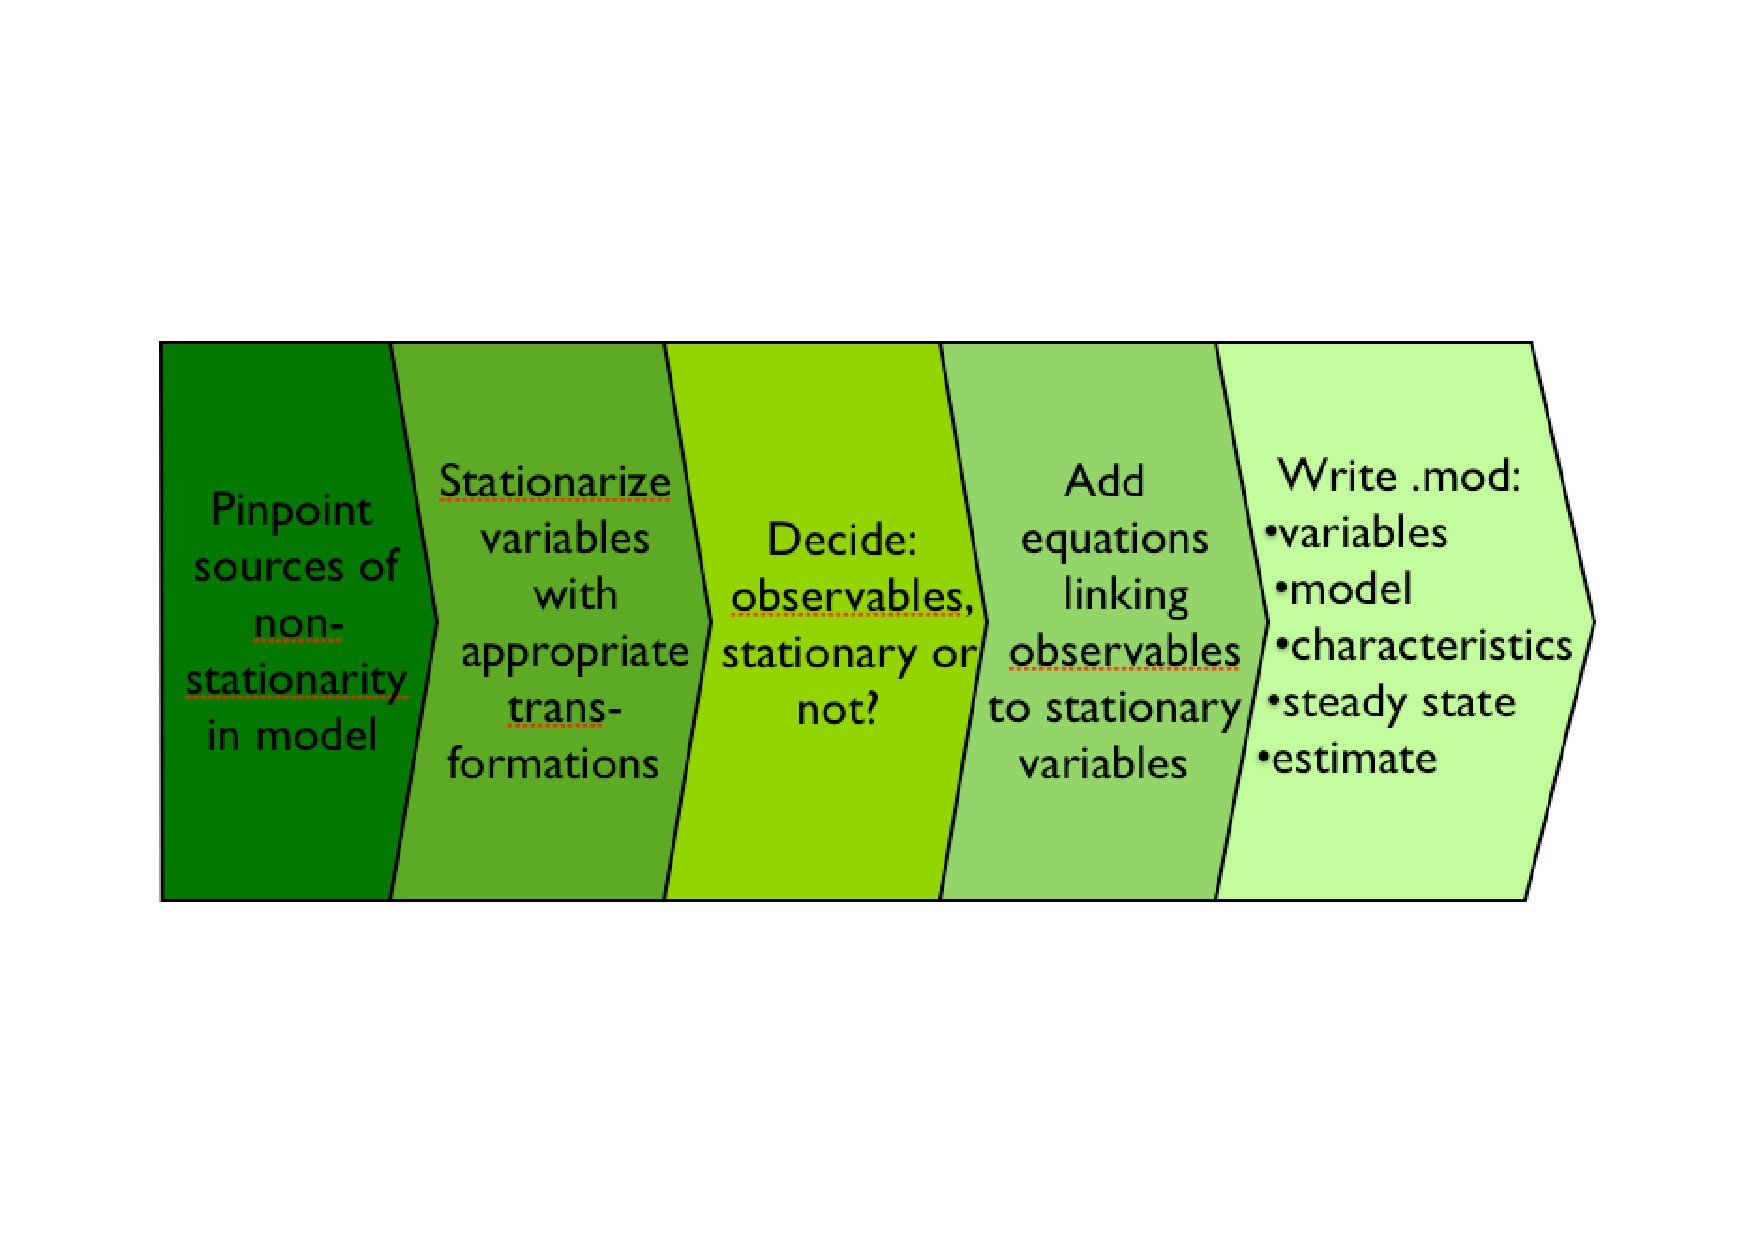
\includegraphics[width=1.0\textwidth]{P_flowest} 
\end{center} 
\caption[Steps of model estimation]{At a high level, there are five basic steps to translate a model into Dynare for successful estimation.} 
\end{figure}\\

\section{Interpreting output}

As in the case of model solution and simulation, Dynare returns both tabular and graphical output. On the basis of the options entered in the example .mod file above, Dynare will display the following results.\\

\subsection{Tabular results}
The first results to be displayed (and calculated from a chronological standpoint) are the steady state results. Note the dummy values of 1 for the non-stationary variables Y\_obs and P\_obs. These results are followed by the eigenvalues of the system, presented in the order in which the endogenous variables are declared at the beginning of the .mod file (** is this true?). The table of eigenvalues is completed with a statement about the Blanchard-Kahn condition being met - hopefully!\\

The next set of results are for the numerical iterations necessary to find the posterior mode, as explained in more details in Chapter \ref{ch:estadv}. The improvement from one iteration to the next reaches zero, Dynare give the value of the objective function (the posterior Kernel) at the mode and displays two important table summarizing results from posterior maximization.\\

The first table summarizes results for parameter values. It includes: prior means, posterior mode, standard deviation and t-stat of the mode (based on the assumption of a Normal, probably erroneous when undertaking Bayesian estimation, as opposed to standard maximum likelihood), as well as the prior distribution and standard deviation (pstdev). It is followed by a second table summarizing the same results for the shocks. (** what does it mean when shocks have pstdev Inf?)\\

\subsection{Graphical results}
(** intersperse screen shots below as each output is discussed)\\

The first figure comes up soon after launching Dynare as little computation is necessary to generate it. The figure returns a graphical representation of the priors for each parameter of interest. \\

The second set of figures displays ``MCMC univariate diagnostics'', where MCMC stands for Monte Carlo Markov Chains. This is the main source of feedback to gain confidence, or spot a problem, with results. Recall that Dynare completes several runs of Metropolis-Hastings simulations (as many as determined in the option \texttt{mh\_nblocks}, each time starting from a different initial value). If the results from one chain are sensible, and the optimizer did not get stuck in an odd area of the parameter subspace, two things should happen. First, results within any of the however many iterations of Metropolis-Hastings simulation should be similar. And second, results between the various chains should be close. This is the idea of what the MCMC diagnostics track. \\

More specifically, the red and blue lines on the charts represent specific measures of the parameter vectors both within and between chains. For the results to be sensible, these should be relatively constant (although there will always be some variation) and they should converge. Dynare reports three measures: ``interval'', being constructed from an 80\% confidence interval around the parameter mean, ``m2'', being a measure of the variance and ``m3'' based on third moments. In each case, Dynare reports both the within and the between chains measures. The figure entitled ``multivariate diagnostic'' presents results of the same nature, except that they reflect an aggregate measure based on the eigenvalues of the variance-covariance matrix of each parameter.\\

In our example above, you can tell that indeed, we obtain convergence and relative stability in all measures of the parameter moments. Note that the horizontal axis represents the number of Metropolis-Hastings iterations that have been undertaken, and the vertical axis the measure of the parameter moments, with the first, corresponding to the measure at the initial value of the Metropolis-Hastings iterations.\\

\textsf{\textbf{TIP!}} If the plotted moments are highly unstable or do not converge, you may have a problem of poor priors. It is advisable to redo the estimation with different priors. If you have trouble coming up with a new prior, try starting with a uniform and relatively wide prior and see where the data leads the posterior distribution. Another approach is to undertake a greater number of Metropolis-Hastings simulations.\\

The first to last figure - figure 6 in our example - displays the most interesting set of results, towards which most of the computations undertaken by Dynare are directed: the posterior distribution. In fact, the figure compares the posterior to the prior distribution (black vs. grey lines). In addition, on the posterior distribution, Dynare plots a green line which represents the posterior mode.\\

\textsf{\textbf{TIP!}} These graphs are not highly relevant and interesting for the results they display, but also as tools to detect problems or build additional confidence in your results. First, the prior and the posterior distributions should not be excessively different. Second, the posterior distributions should be close to normal, or at least not display a shape that is clearly non-normal. Third, the green mode (calculated from the numerical optimization of the posterior kernel) should not be too far away from the mode of the posterior distribution. If not, it is advisable to undertake a greater number of Metropolis-Hastings simulations. \\

The last figure returns the smoothed estimated shocks in a useful illustration to eye-ball the plausibility of the size and frequency of the shocks. The horizontal axis, in this case, represents the number of periods in the sample. One thing to check is the fact that shocks should be centered around zero. That is indeed the case for our example. \\

 






